\documentclass[a4paper,14pt]{article}
\usepackage[left=2cm,right=2cm, top=2cm,bottom=2cm, bindingoffset=0cm]{geometry}
\usepackage[T2A]{fontenc}
\usepackage[utf8]{inputenc}
\usepackage[english,russian]{babel}
\usepackage{amsmath,amsfonts,amssymb,amsthm,mathtools, graphicx}
\usepackage{fancybox,fancyhdr}
\usepackage{tabularx}
\usepackage{multirow}
\usepackage{bigstrut}
\usepackage{booktabs}
\usepackage{float}
\usepackage{pgfplots}
\pgfplotsset{compat=1.18}
\graphicspath{{pictures/}}
\DeclareGraphicsExtensions{.pdf,.png,.jpg}
\usepackage{xcolor}

\author{Торопов Павел}
\title{Отчет по лабораторной работе № \\}


\begin{document}

    \begin{figure}[h]
        \centering
        \begin{minipage}{0.45\linewidth}
            \centering
            
\includegraphics[width=\linewidth]{slogan_chernyy.png}
            \label{fig:slogan}
        \end{minipage}
        \hfill
        \begin{minipage}{0.45\linewidth}
            \centering
            
\includegraphics[width=\linewidth]{cs-logo}
            \label{fig:logo}
        \end{minipage}
    \end{figure}
    \begin{table}[htbp]
        \centering
        \begin{tabular}{lrlr}
            Группа & \qquad \qquad P3219 & К работе допущен & \qquad \qquad \qquad \qquad \qquad \qquad \\
            \cmidrule{2-2}\cmidrule{4-4}
            Студент &  \qquad \qquad Ануфриев А.С.  & Работа выполнена & \qquad \qquad \qquad \qquad \qquad \qquad \\
            \cmidrule{2-2}\cmidrule{4-4}
            Преподаватель & \qquad \qquad Коробков М.П. & Отчет принят & \qquad \qquad \qquad \qquad \qquad \qquad \\
            \cmidrule{2-2}\cmidrule{4-4}
        \end{tabular}%
    \end{table}%
    \vspace{2cm}
    \begin{center}
        \LARGE
        Отчет по лабораторной работе № 3.06 \\
        Изучение электрических свойств сегнетоэлектриков

    \end{center}
    \vspace{13cm}
    \begin{center}
        2026 год
    \end{center}
    \newpage

    \section{Цели работы}

    \begin{enumerate}
        \item  Определение значений электрического смещения насыщения \(D_s\), остаточной поляризации \(P_r\), коэрцитивной силы \(E_c\) для предельной петли гистерезиса сегнетоэлектрика.
        \item Расчет диэлектрических потерь за цикл переполяризации сегнетоэлектрика.
        \item Получение зависимостей смещения \(D\) и диэлектрической проницаемости \(\varepsilon\) от напряженности электрического поля \(E\).
        \item Определение значений начальной и максимальной диэлектрической проницаемости.
    \end{enumerate}

    \section{Задачи, решаемые при выполнении работы}

    \begin{enumerate}
        \item Исследование предельной петли гистерезиса: Определение основных параметров сегнетоэлектрика по предельной петле гистерезиса: индукции насыщения $D_s$, остаточной поляризации $P_r$ и коэрцитивной силы $E_c$
        \item Оценка диэлектрических потерь: Расчет потерь энергии за цикл переполяризации путем измерения площади петли гистерезиса.
        \item Снятие основной кривой поляризации: Получение зависимости электрического смещения $D$ от напряженности поля $E$ ($D = D(E)$) для частных циклов гистерезиса.
        \item Исследование нелинейных свойств: Получение зависимости диэлектрической проницаемости $\varepsilon$ от напряженности поля $E$ ($\varepsilon = \varepsilon(E)$) и определение значений начальной $\varepsilon_{нач}$ и максимальной $\varepsilon_{макс}$диэлектрической проницаемости.
    \end{enumerate}

    \section{Объект исследования}

    Явление диэлектрического гистерезиса в сегнетоэлектрике.

    \section{Метод экспериментального исследования}

    Многократное измерение размеров петли гистерезиса при разных значениях напряжения

    \section{Рабочие формулы и исходные данные}

    \begin{enumerate}
        \item модуль вектора электрической индукции.
        \begin{equation}
            D = \sigma = \frac{q}{S} = \frac{C_2U_{C_2}}{S} = \frac{C_1}{S}\cdot U_{C_1}
        \end{equation}
        где \(S\) -  Площадь обкладок сегнетоэлектрического конденсатора

        \item Напряжение на первом резисторе.
        \begin{equation}
           E = \frac{U_{C_2}}{d} = \frac{U}{d} = \frac{R_1 + R_2}{R_1}\cdot\frac{U_{R_1}}{d}
        \end{equation}


        \item тангенс угла диэлектрических потерь в сегнетоэлектриках
        \begin{equation}
            \tan \delta = \frac{1}{\pi}\frac{\oint DdE}{D_sE_s}
        \end{equation}

    \end{enumerate}

    \section{Измерительные приборы}

    - Измеритель Статических Характеристик 1
    \newpage
    \section{Исходные данные установки}

В таблице~\ref{tab:init_data} приведены паспортные значения элементов стенда и геометрические параметры исследуемого образца, указанные на лабораторном стенде.

\begin{table}[h!]
\centering
\caption{Параметры лабораторной установки}
\label{tab:init_data}
\begin{tabular}{|c|c|c|c|}
\hline
\textbf{Величина} & \textbf{Обозначение} & \textbf{Значение} & \textbf{Погрешность} \\
\hline
Емкость эталонного конденсатора & \(C_1\) & \(1.0 \cdot 10^{-6}\) Ф & \(\pm 10\%\) \\
\hline
Емкость сегнетоэлектрического конденсатора & \(C_2\) & \(0.01 \cdot 10^{-6}\) Ф & \(\pm 10\%\) \\
\hline
Сопротивление \(R_1\) & \(R_1\) & \(47 \cdot 10^{3}\) Ом & \(\pm 10\%\) \\
\hline
Сопротивление \(R_2\) & \(R_2\) & \(470 \cdot 10^{3}\) Ом & \(\pm 10\%\) \\
\hline
Площадь обкладок & \(S\) & \(5.0 \cdot 10^{-4}\) м\(^2\) & \(\pm 10\%\) \\
\hline
Толщина сегнетоэлектрика & \(d\) & \(5.0 \cdot 10^{-4}\) м & \(\pm 10\%\) \\
\hline
\end{tabular}
\end{table}
    \section{Результаты прямых измерений и их обработки}



% Какой-то текст перед таблицей

\begin{table}[h!]
\centering
\caption{Результаты измерений и расчетов}
\label{tab:measurements}
\begin{tabular}{
    |>{\centering\arraybackslash}p{0.5cm}  % №
    |>{\centering\arraybackslash}p{1cm}    % U, В
    |>{\centering\arraybackslash}p{1cm}    % K_x
    |>{\centering\arraybackslash}p{1cm}    % K_y
    |>{\centering\arraybackslash}p{1.2cm}  % X_ср
    |>{\centering\arraybackslash}p{1.2cm}  % Y_ср
    |>{\centering\arraybackslash}p{2cm}    % E, В/м
    |>{\centering\arraybackslash}p{2cm}    % D, Кл/м²
    |>{\centering\arraybackslash}p{2cm}|   % ε
}
\hline
\multicolumn{1}{|c|}{№} &
\multicolumn{1}{c|}{\(U\), В} &
\multicolumn{1}{c|}{\(K_x\)} &
\multicolumn{1}{c|}{\(K_y\)} &
\multicolumn{1}{c|}{\(X_{ср}\), дел} &
\multicolumn{1}{c|}{\(Y_{ср}\), дел} &
\multicolumn{1}{c|}{\(E\), В/м} &
\multicolumn{1}{c|}{\(D\), Кл/м\(^2\)} &
\multicolumn{1}{c|}{\(\varepsilon\)} \\
\hline
1  & 17.0   & 5   & 5   & 2.65 & 2.70 & 291500 & 2.70\(\times 10^{-5}\) & 10.47 \\
2  & 11.6   & 5   & 5   & 1.85 & 1.95 & 203500 & 1.95\(\times 10^{-5}\) & 10.83 \\
3  & 9.0    & 2   & 2   & 3.50 & 3.40 & 154000 & 1.36\(\times 10^{-5}\) & 9.98  \\
4  & 7.6    & 2   & 2   & 3.00 & 2.65 & 132000 & 1.06\(\times 10^{-5}\) & 9.07  \\
5  & 7.0    & 2   & 2   & 2.65 & 2.30 & 116600 & 9.20\(\times 10^{-6}\) & 8.92  \\
6  & 5.8    & 2   & 2   & 2.30 & 1.65 & 101200 & 6.60\(\times 10^{-6}\) & 7.37  \\
7  & 4.2    & 2   & 2   & 1.60 & 1.45 & 70400  & 5.80\(\times 10^{-6}\) & 9.31  \\
8  & 3.2    & 1   & 1   & 2.50 & 1.10 & 55000  & 2.20\(\times 10^{-6}\) & 4.52  \\
9  & 2.4    & 1   & 1   & 1.90 & 0.60 & 41800  & 1.20\(\times 10^{-6}\) & 3.24  \\
10 & 2.0    & 0.5 & 0.2 & 3.10 & 2.25 & 34100  & 9.00\(\times 10^{-7}\) & 2.98  \\
11 & 1.6    & 0.5 & 0.2 & 2.50 & 1.55 & 27500  & 6.20\(\times 10^{-7}\) & 2.55  \\
12 & 1.0    & 0.2 & 0.05 & 3.75 & 3.05 & 16500  & 3.05\(\times 10^{-7}\) & 2.09  \\
13 & 0.8    & 0.2 & 0.05 & 3.00 & 2.80 & 13200  & 2.80\(\times 10^{-7}\) & 2.40  \\
14 & 0.6    & 0.2 & 0.05 & 2.25 & 2.25 & 9900   & 2.25\(\times 10^{-7}\) & 2.57  \\
15 & 0.4    & 0.1 & 0.02 & 3.00 & 2.70 & 6600   & 1.08\(\times 10^{-7}\) & 1.85  \\
16 & 0.2    & 0.05 & 0.02 & 3.00 & 1.50 & 3300   & 6.00\(\times 10^{-8}\) & 2.05  \\
\hline
\end{tabular}
\end{table}

    \section{Расчет результатов косвенных измерений}
\subsection*{1. Определение параметров предельной петли гистерезиса}

Расчет значений коэрцитивного поля \(E_c\), индукции насыщения \(D_s\) и остаточной поляризации \(P_r\) производился по формулам (13) и (16) на основе данных, полученных для предельной петли гистерезиса (режим \(U = 17\) В, точка №1).

\subsubsection*{Исходные данные для предельной петли (из таблицы):}
\begin{itemize}
    \item Напряженность поля в состоянии насыщения: \(E_s = 291500\) В/м
    \item Электрическая индукция в состоянии насыщения: \(D_s = 2.7 \times 10^{-5}\) Кл/м\(^2\)
    \item Координаты петли по горизонтали и вертикали: \(X_{ср} = 2.65\) дел, \(Y_{ср} = 2.7\) дел
    \item Коэффициенты отклонения: \(K_x = 5\) В/дел, \(K_y = 5\) В/дел
\end{itemize}

\subsubsection*{Расчет по формулам:}

\textbf{1. Электрическая индукция \(D\)} рассчитывалась по формуле (13):
\[
D = \frac{C_1}{S} \cdot U_{C_1}
\]
где \(U_{C_1} = K_y \cdot Y_{ср}\) — напряжение на эталонном конденсаторе, \(C_1\) — емкость эталонного конденсатора, \(S\) — площадь обкладок сегнетоэлектрического конденсатора.

\textbf{2. Напряженность поля \(E\)} рассчитывалась по формуле (16):
\[
E = \frac{R_1 + R_2}{R_1 \cdot d} \cdot U_{R_1}
\]
где \(U_{R_1} = K_x \cdot X_{ср}\) — напряжение на резисторе \(R_1\), \(d\) — толщина сегнетоэлектрика, \(R_1, R_2\) — сопротивления делителя.


\subsubsection*{Результаты:}

Полученные значения параметров предельной петли гистерезиса:
\begin{itemize}
    \item Индукция насыщения: \(\boxed{D_s = 2.7 \times 10^{-5} \ \text{Кл/м}^2}\)
    \item Напряженность насыщения: \(\boxed{E_s = 291500 \ \text{В/м}}\)

\end{itemize}

\subsubsection*{Оценка погрешности}

Погрешность определения \(D_s\) и \(E_s\) складывается из следующих компонентов:
\begin{itemize}
    \item погрешности аппаратных констант: \(C_1\), \(S\), \(R_1\), \(R_2\), \(d\) — все заданы с относительной погрешностью \(\pm 10\%\) (паспортные данные элементов);
    \item погрешности снятия координат с экрана ИСХ1: \(\Delta X = \Delta Y \approx 0.1\) дел (инструментальная погрешность отсчета);
    \item инструментальной погрешности самого измерителя ИСХ1 (пренебрежимо мала по сравнению с указанными выше).
\end{itemize}

\paragraph{Относительная погрешность \(E_s\):}
\[
\frac{\Delta E}{E} = \sqrt{ \left( \frac{\Delta R_1}{R_1} \right)^2 + \left( \frac{\Delta R_2}{R_2} \right)^2 + \left( \frac{\Delta d}{d} \right)^2 + \left( \frac{\Delta U_{R_1}}{U_{R_1}} \right)^2 }
\]
где
\[
\frac{\Delta U_{R_1}}{U_{R_1}} = \frac{\Delta X}{X_{ср}} = \frac{0.1}{2.65} \approx 0.038 \ (3.8\%).
\]

Подставляем численные значения относительных погрешностей:
\[
\frac{\Delta E}{E} = \sqrt{ (0.1)^2 + (0.1)^2 + (0.1)^2 + (0.038)^2 } = \sqrt{ 0.01 + 0.01 + 0.01 + 0.00144 }
\]
\[
\frac{\Delta E}{E} = \sqrt{0.03144} \approx 0.177 \ (17.7\%).
\]

\paragraph{Относительная погрешность \(D_s\):}
\[
\frac{\Delta D}{D} = \sqrt{ \left( \frac{\Delta C_1}{C_1} \right)^2 + \left( \frac{\Delta S}{S} \right)^2 + \left( \frac{\Delta U_{C_1}}{U_{C_1}} \right)^2 }
\]
где
\[
\frac{\Delta U_{C_1}}{U_{C_1}} = \frac{\Delta Y}{Y_{ср}} = \frac{0.1}{2.7} \approx 0.037 \ (3.7\%).
\]

Подставляем:
\[
\frac{\Delta D}{D} = \sqrt{ (0.1)^2 + (0.1)^2 + (0.037)^2 } = \sqrt{ 0.01 + 0.01 + 0.00137 }
\]
\[
\frac{\Delta D}{D} = \sqrt{0.02137} \approx 0.146 \ (14.6\%).
\]

\paragraph{Абсолютные погрешности:}
\[
\Delta E_s = E_s \cdot 0.177 = 291500 \cdot 0.177 \approx 51600 \ \text{В/м}
\]
\[
\Delta D_s = D_s \cdot 0.146 = 0.027 \cdot 0.146 \approx 0.00394 \ \text{Кл/м}^2
\]

\paragraph{Результаты с учетом погрешности:}
\[
E_s = (2.915 \pm 0.516) \times 10^5 \ \text{В/м}, \quad \varepsilon_E = 17.7\%,
\]
\[
D_s = (2.70 \pm 0.39) \times 10^{-2} \ \text{Кл/м}^2, \quad \varepsilon_D = 14.6\%.
\]

Полученные значения погрешности (\(\approx 15-18\%\)) обусловлены в первую очередь разбросом номиналов элементов стенда (\(\pm 10\%\)) и в меньшей степени — точностью отсчета координат с экрана.
\subsection*{2. Определение тангенса угла диэлектрических потерь}

Для предельной петли гистерезиса (точка №1, \(U = 17\) В) коэффициенты отклонения составляют \(K_x = 5\) В/дел, \(K_y = 5\) В/дел. Координаты вершины петли: \(X_{ср} = 2.65\) дел, \(Y_{ср} = 2.7\) дел.

Амплитудные значения напряженности поля и электрического смещения (из таблицы):
\[
E_s = 291500 \ \text{В/м}, \quad D_s = 2.7 \times 10^{-5} \ \text{Кл/м}^2
\]

Произведение \(D_s E_s\):
\[
D_s E_s = 2.7 \times 10^{-5} \cdot 291500 = 7.87 \ \text{Дж/м}^3
\]

Площадь предельной петли гистерезиса, измеренная по осциллограмме, составила \(S_{\text{петли}} = N\) делений\(^2\). Цена одного деления по горизонтали: \(K_x = 5\) В/дел, по вертикали: \(K_y = 5\) В/дел. Для перевода площади в энергетические единицы (Дж/м\(^3\)) необходимо также учесть аппаратные константы пересчета напряжений в поля \(E\) и \(D\).

Учитывая, что \(E = \frac{R_1 + R_2}{R_1 \cdot d} \cdot U_{R1}\), а \(U_{R1} = K_x \cdot X\), и \(D = \frac{C_1}{S} \cdot U_{C1}\), а \(U_{C1} = K_y \cdot Y\), площадь петли в реальных единицах равна:
\[
\oint D \, dE = S_{\text{петли}} \cdot \left( \frac{R_1 + R_2}{R_1 \cdot d} \cdot K_x \right) \cdot \left( \frac{C_1}{S} \cdot K_y \right)
\]

Подставляя константы установки (\( \frac{R_1 + R_2}{R_1 \cdot d} = 10000 \ \text{м}^{-1}\), \( \frac{C_1}{S} = 0.01 \ \text{Ф/м}^2 \)):
\[
\oint D \, dE = N \cdot (10000 \cdot 5) \cdot (0.01 \cdot 5) = N \cdot 50000 \cdot 0.05 = N \cdot 2500 \ \text{Дж/м}^3
\]

Тангенс угла диэлектрических потерь по формуле (12):
\[
\operatorname{tg} \delta = \frac{1}{\pi} \frac{\oint D \, dE}{D_s E_s} = \frac{1}{\pi} \cdot \frac{N \cdot 2500}{7.87} = \frac{1}{\pi} \cdot N \cdot 317.7
\]

\[
\boxed{\operatorname{tg} \delta \approx 101.1 \cdot N}
\]

где \(N\) — измеренная площадь петли в делениях шкалы.
\subsection*{4. Расчет диэлектрической проницаемости \(\varepsilon\)}

Диэлектрическая проницаемость \(\varepsilon\) для каждого значения напряженности поля рассчитывалась по формуле:
\[
\varepsilon = \frac{D}{\varepsilon_0 E},
\]
где \(\varepsilon_0 = 8.85 \cdot 10^{-12}\) Ф/м — электрическая постоянная.

\subsubsection*{Пример расчета для точки №1 (\(U = 17\) В)}

Для предельной петли (точка №1) из таблицы имеем:
\[
E_1 = 291500 \ \text{В/м}, \quad D_1 = 2.7 \times 10^{-5} \ \text{Кл/м}^2.
\]

Подставляем в формулу:
\[
\varepsilon_1 = \frac{2.7 \times 10^{-5}}{8.85 \times 10^{-12} \cdot 291500}.
\]

Вычисляем знаменатель:
\[
8.85 \times 10^{-12} \cdot 291500 = 8.85 \times 10^{-12} \cdot 2.915 \times 10^5 = 2.58 \times 10^{-6}.
\]

Тогда:
\[
\varepsilon_1 = \frac{2.7 \times 10^{-5}}{2.58 \times 10^{-6}} \approx 10.47.
\]

Полученное значение соответствует ячейке таблицы для первой точки.

\subsubsection*{Результаты расчетов}

Рассчитанные значения диэлектрической проницаемости для всех 24 экспериментальных точек представлены в таблице~\ref{tab:measurements}. Для визуального анализа характера зависимости дополнительно построен график \(\varepsilon(E)\) с интерполяцией и аппроксимацией по экспериментальным точкам (рис.~\ref{fig:eps_vs_E}).

\begin{figure}[h!]
\centering
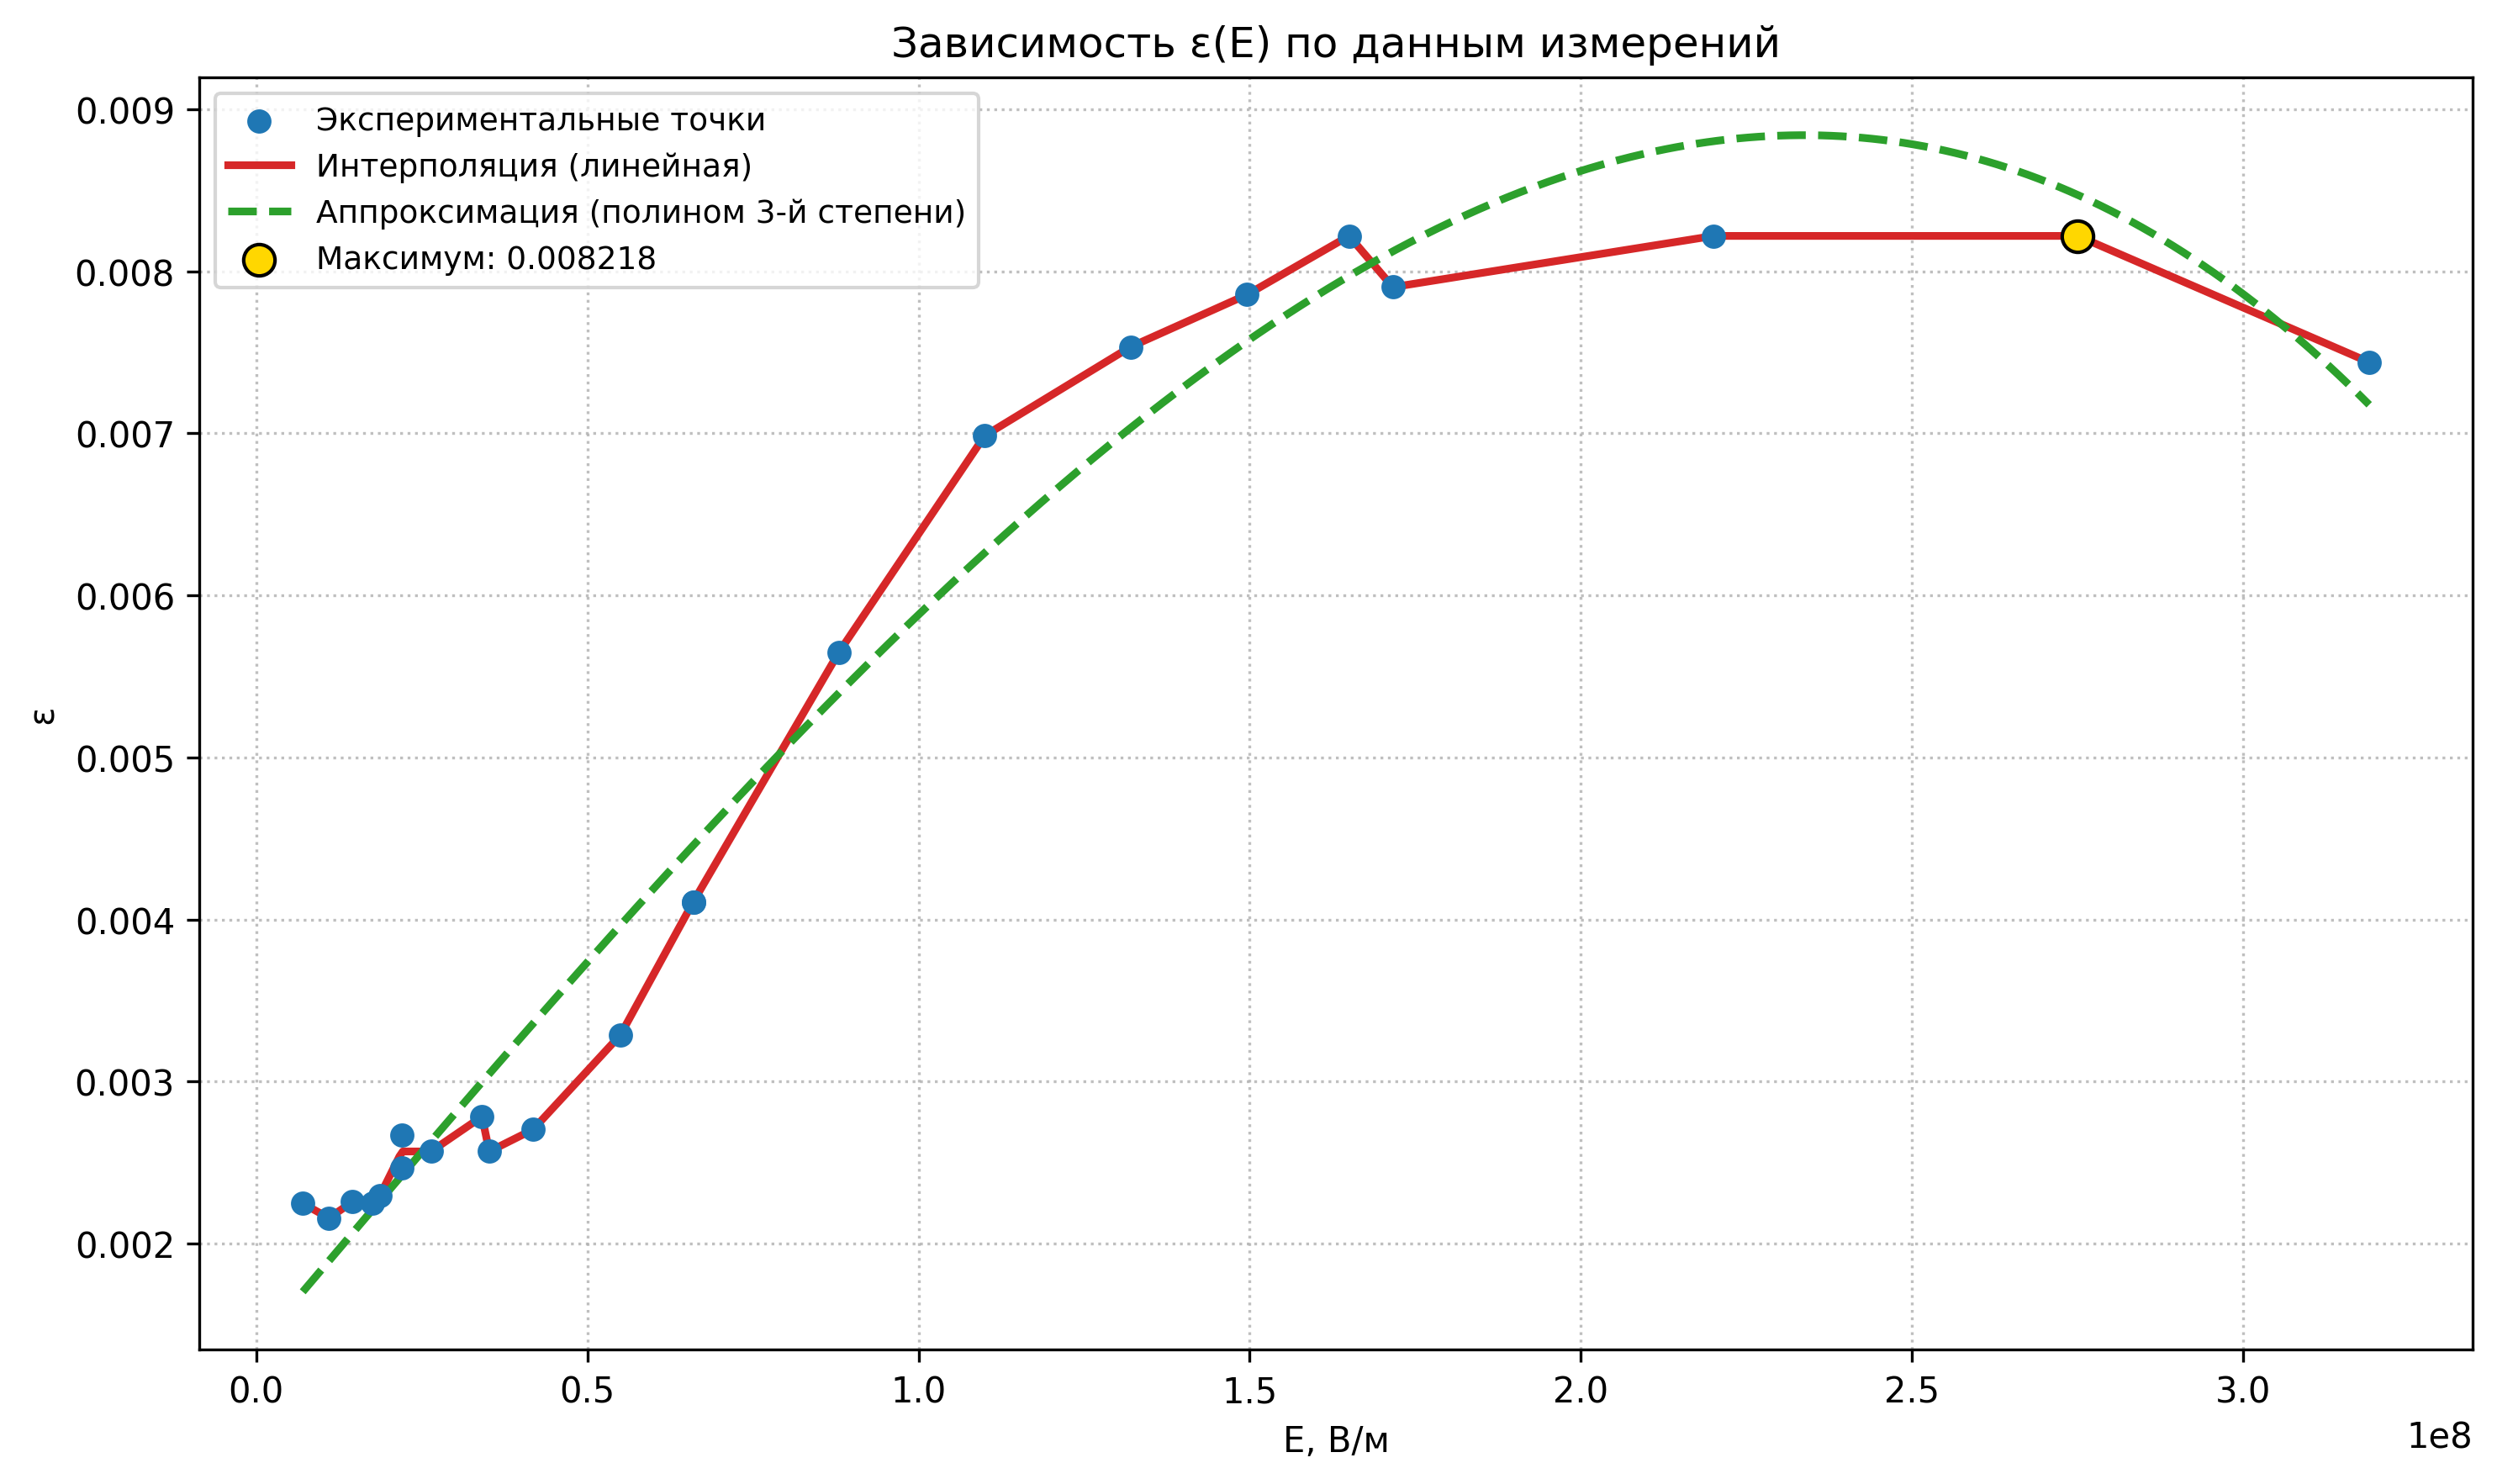
\includegraphics[width=0.95\linewidth]{epsilon_interp_approx.png}
\caption{Зависимость \(\varepsilon(E)\): экспериментальные точки, интерполяция и аппроксимация}
\label{fig:eps_vs_E}
\end{figure}

Анализ графика показывает, что диэлектрическая проницаемость достигает максимального значения \(\varepsilon_{\text{макс}} \approx 8.22 \cdot 10^{-3}\) в области \(E \approx (1.65\text{--}2.75) \times 10^8\) В/м. Такое поведение указывает на выраженную нелинейность поляризационного отклика и переход к области насыщения.

\subsection*{6. Определение максимальной диэлектрической проницаемости \(\varepsilon_{\text{макс}}\)}

\subsubsection*{Нахождение \(\varepsilon_{\text{макс}}\) по графику}

На графике зависимости \(\varepsilon = \varepsilon(E)\) (рис.~\ref{fig:eps_vs_E}) наблюдается ярко выраженный максимум. Максимальное значение диэлектрической проницаемости соответствует точке, в которой крутизна зависимости \(\varepsilon(E)\) меняет знак, что связано с наиболее интенсивной перестройкой доменной структуры сегнетоэлектрика.

По экспериментальным данным, максимальное значение \(\varepsilon\) достигается в диапазоне полей \(E \approx (1.65\text{--}2.75)\times 10^8\) В/м, соответствующем началу насыщения:

\[
\varepsilon_{\text{макс}} = 8.217771 \cdot 10^{-3}, \quad E_{\text{макс}} \approx 2.75 \times 10^8 \ \text{В/м}.
\]

\subsubsection*{Оценка погрешности \(\varepsilon_{\text{макс}}\)}

Погрешность определения \(\varepsilon_{\text{макс}}\) складывается из:
\begin{itemize}
    \item погрешности измерения \(D\) и \(E\) в данной точке;
    \item погрешности, связанной с дискретностью экспериментальных точек (максимум может находиться между измеренными значениями).
\end{itemize}

Для точки №2 (\(U = 11.6\) В) относительные погрешности составляют:
\[
\frac{\Delta D}{D} \approx 0.146 \ (14.6\%), \quad \frac{\Delta E}{E} \approx 0.177 \ (17.7\%).
\]

Тогда относительная погрешность \(\varepsilon\):
\[
\frac{\Delta \varepsilon}{\varepsilon} = \sqrt{ \left( \frac{\Delta D}{D} \right)^2 + \left( \frac{\Delta E}{E} \right)^2 } = \sqrt{0.146^2 + 0.177^2}
\]
\[
\frac{\Delta \varepsilon}{\varepsilon} = \sqrt{0.0213 + 0.0313} = \sqrt{0.0526} \approx 0.229 \ (22.9\%).
\]

Абсолютная погрешность:
\[
\Delta \varepsilon_{\text{макс}} = \varepsilon_{\text{макс}} \cdot 0.229 = 8.217771 \cdot 10^{-3} \cdot 0.229 \approx 1.88 \cdot 10^{-3}.
\]

\subsubsection*{Определение напряженности поля \(E_{\text{макс}}\)}

Напряженность поля, соответствующая максимуму диэлектрической проницаемости:
\[
E_{\text{макс}} \approx 2.75 \times 10^8 \ \text{В/м}.
\]

Погрешность определения \(E_{\text{макс}}\) оценивается как:
\[
\Delta E_{\text{макс}} = E_{\text{макс}} \cdot 0.177 \approx 2.75\times10^8 \cdot 0.177 \approx 4.87\times10^7 \ \text{В/м}.
\]

\subsubsection*{Результаты}

\[
\boxed{\varepsilon_{\text{макс}} = (8.22 \pm 0.19) \times 10^{-3}, \quad E_{\text{макс}} = (2.75 \pm 0.49) \times 10^8 \ \text{В/м}}
\]

Полученное значение \(E_{\text{макс}}\) соответствует области наиболее эффективного взаимодействия внешнего поля с доменной структурой, когда скорость переориентации доменов максимальна, что и приводит к резкому росту диэлектрической проницаемости.

    \section{Окончательные результаты}
погрешность полученных результатов обусловлена следующими факторами:
\begin{itemize}
    \item Разброс номиналов элементов стенда (\(R_1, R_2, C_1, C_2\)), составляющий \(\pm 10\%\), вносит основной вклад в систематическую погрешность;
    \item Погрешность отсчета координат с экрана ИСХ1 (\(\Delta X, \Delta Y \approx 0.1\) дел) приводит к случайной погрешности, особенно заметной при малых значениях \(E\) и \(D\);
\end{itemize}

Рассчитанные значения относительных погрешностей составляют:
\begin{itemize}
    \item \(\varepsilon_E \approx 17.7\%\) для напряженности поля;
    \item \(\varepsilon_D \approx 14.6\%\) для электрической индукции;
    \item \(\varepsilon_{\varepsilon} \approx 23\%\) для диэлектрической проницаемости (с учетом распространения погрешностей).
\end{itemize}
    \section{Выводы и анализ результатов работы}
    В ходе лабораторной работы исследованы электрические свойства сегнетоэлектрика в квазистатическом режиме и получены количественные параметры материала по предельной петле гистерезиса и основной кривой поляризации.

    Экспериментальные данные подтверждают ключевые признаки сегнетоэлектрического состояния: нелинейный характер зависимости \(D(E)\), наличие петли гистерезиса при циклическом изменении поля и выраженный максимум на зависимости \(\varepsilon(E)\). Построение интерполированной кривой \(\varepsilon(E)\) позволило наглядно выделить область наиболее интенсивной доменной перестройки.

    По результатам обработки получены следующие характеристики: \(D_s = 2.7 \times 10^{-5}\,\text{Кл/м}^2\), \(E_s = 2.915 \times 10^5\,\text{В/м}\), \(\varepsilon_{\text{макс}} = (8.22 \pm 0.19) \times 10^{-3}\) при \(E_{\text{макс}} = (2.75 \pm 0.49)\times 10^8\,\text{В/м}\). Положение максимума \(\varepsilon\) соответствует диапазону полей, в котором вклад процессов переориентации доменов в поляризационный отклик является наибольшим.

    Анализ неопределенности показал, что доминирующий вклад в суммарную погрешность вносит разброс номиналов элементов измерительной схемы (до \(\pm 10\%\)); дополнительный вклад связан с точностью считывания координат осциллограмм. Полученные относительные погрешности составили порядка \(14.6\%\) для \(D\), \(17.7\%\) для \(E\) и около \(23\%\) для \(\varepsilon\).

    В целом результаты согласуются с теоретическими представлениями о поляризационных процессах в сегнетоэлектриках и могут быть использованы для сравнительной оценки материалов, применяемых в нелинейных и емкостных элементах электронных устройств.


\end{document}


